%%%%%%%%%%%%%%%%%%%%%%
\begin{frame}{Switching graph topology}
\vskip 0.9cm
In this case the analysis is more complex and depends on more factors.
We can see some of them through an example.
Let's consider the following graphs defined by the matrices:
$$
L_1 = \begin{bmatrix}
	  	1  &  -1  &  0 \\[0.3em]
		0  &  0  &  0  \\[0.3em]
		0  &  0  &  0  \\
	  \end{bmatrix}, \quad
L_2 = \begin{bmatrix}
	  	1  &  -1  &  0 \\[0.3em]
		0  &  1  &  -1  \\[0.3em]
		-2  &  0  &  2  \\
	  \end{bmatrix}, \quad
L_3 = \begin{bmatrix}
	  	0  &  0  &  0 \\[0.3em]
		0  &  1  &  -1  \\[0.3em]
		0  &  0  &  0  \\
	  \end{bmatrix}
$$
Also let $\gamma_1 = \gamma_2 = \gamma_3 = 1$ and let $\Gamma_i$ be defined as
$$
\Gamma_i = \begin{bmatrix}
	  	0_{n \times n}  &  I_n \\[0.3em]
		- L_i  &  - \gamma_i L_i \\
	  	\end{bmatrix}
$$
We note that  {\textcolor{green!40!black}{\fontsize{13}{15}\textbf{$\Gamma_2$ has two zero eigenvalues}}} 
and all the others have negative real parts,
while both  {\textcolor{green!40!black}{\fontsize{13}{15}\textbf{$\Gamma_1$ and $\Gamma_3$ have four zero eigenvalues}}} 
and all the others have negative real parts.
\end{frame}

%%%%%%%%%%%%%%%%%%%%%%
\begin{frame}{Switching graph topology}

\begin{columns}
 \begin{column}{.70\textwidth}
	\begin{center}
		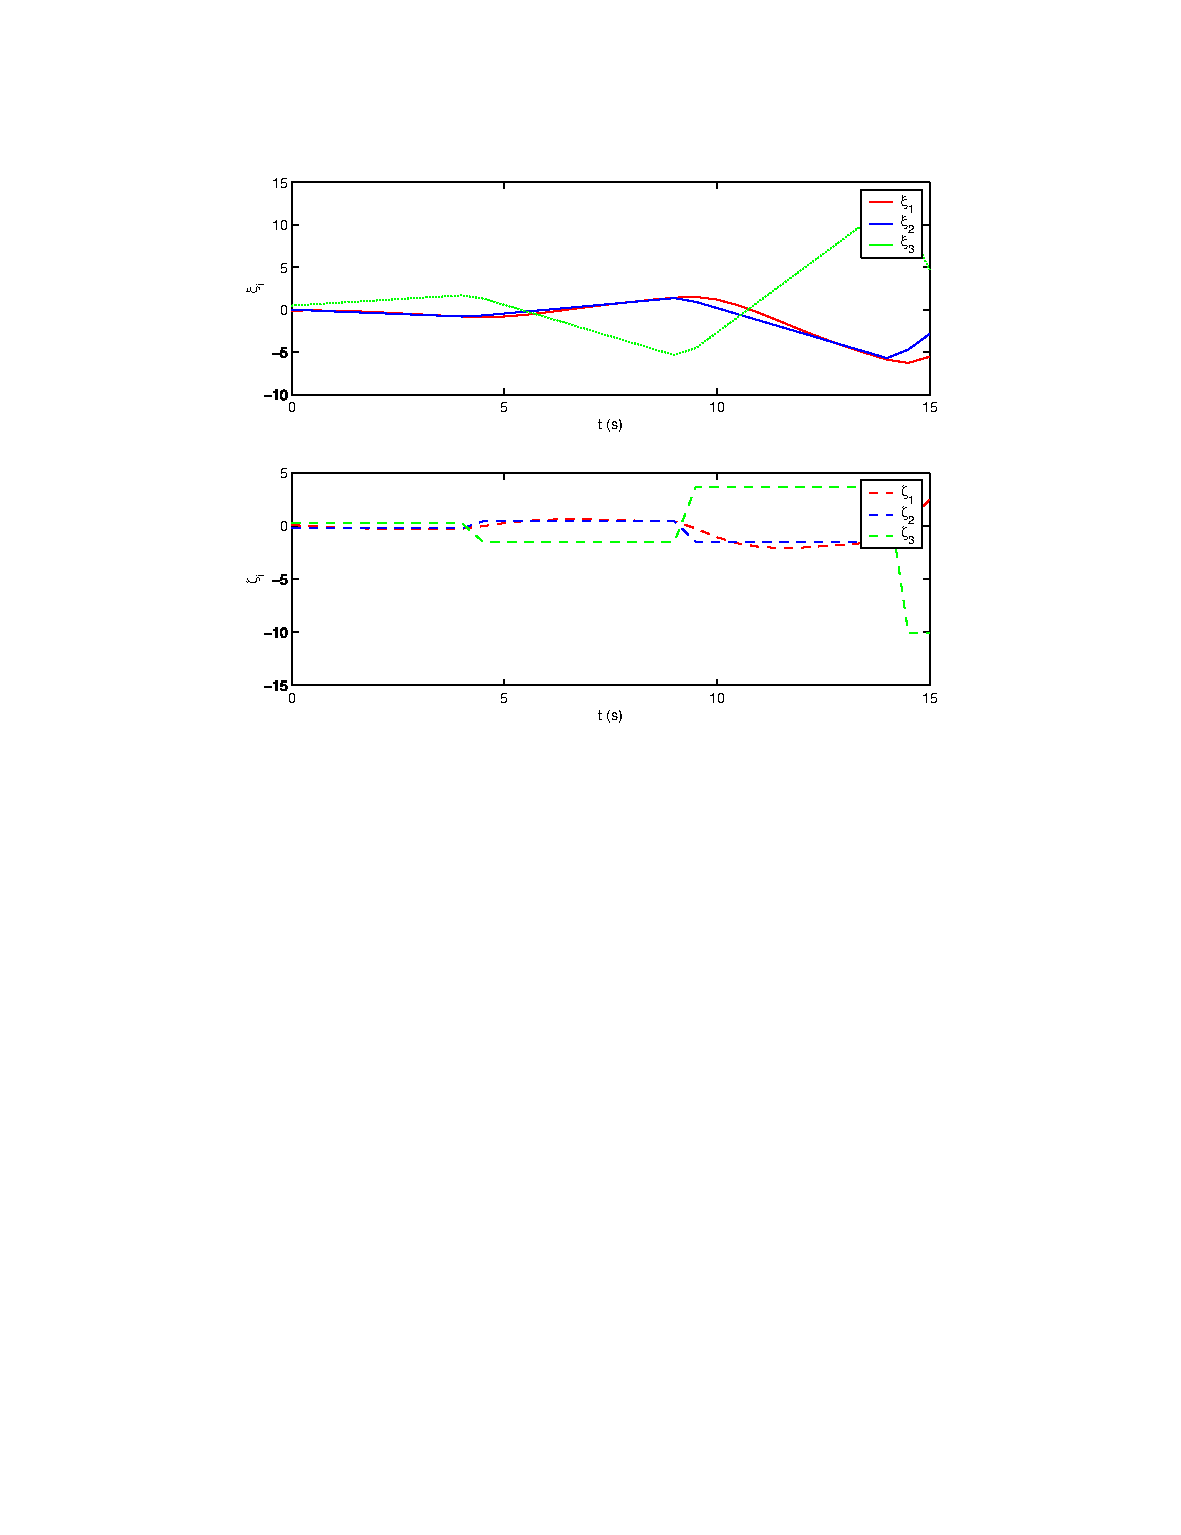
\includegraphics[height=6cm]{images/Switch1.pdf}
	\end{center}
	\vskip 0.3cm
 \end{column}

 \begin{column}{.30\textwidth}
	At each time interval of 5 s we let the information exchange topology be $G_1$ during 90\% of the time 
	and be $G_2$ during the rest of the time. 
	Note that $G_1 \cup G_2$ has a (directed) spanning tree. 
 \end{column}
\end{columns}
Using the {\textcolor{green!40!black}{\fontsize{13}{15}\textbf{first-order consensus}}} protocol, 
{\textcolor{green!40!black}{\fontsize{13}{15}\textbf{consensus can be achieved}}}, 
while {\textcolor{green!40!black}{\fontsize{13}{15}\textbf{consensus cannot be achieved}}} 
using the {\textcolor{green!40!black}{\fontsize{13}{15}\textbf{second-order consensus}}} protocol. 
\vskip 0.3cm

\end{frame}

%%%%%%%%%%%%%%%%%%%%%%
\begin{frame}{Switching graph topology}

\begin{columns}
 \begin{column}{.70\textwidth}
	\begin{center}
		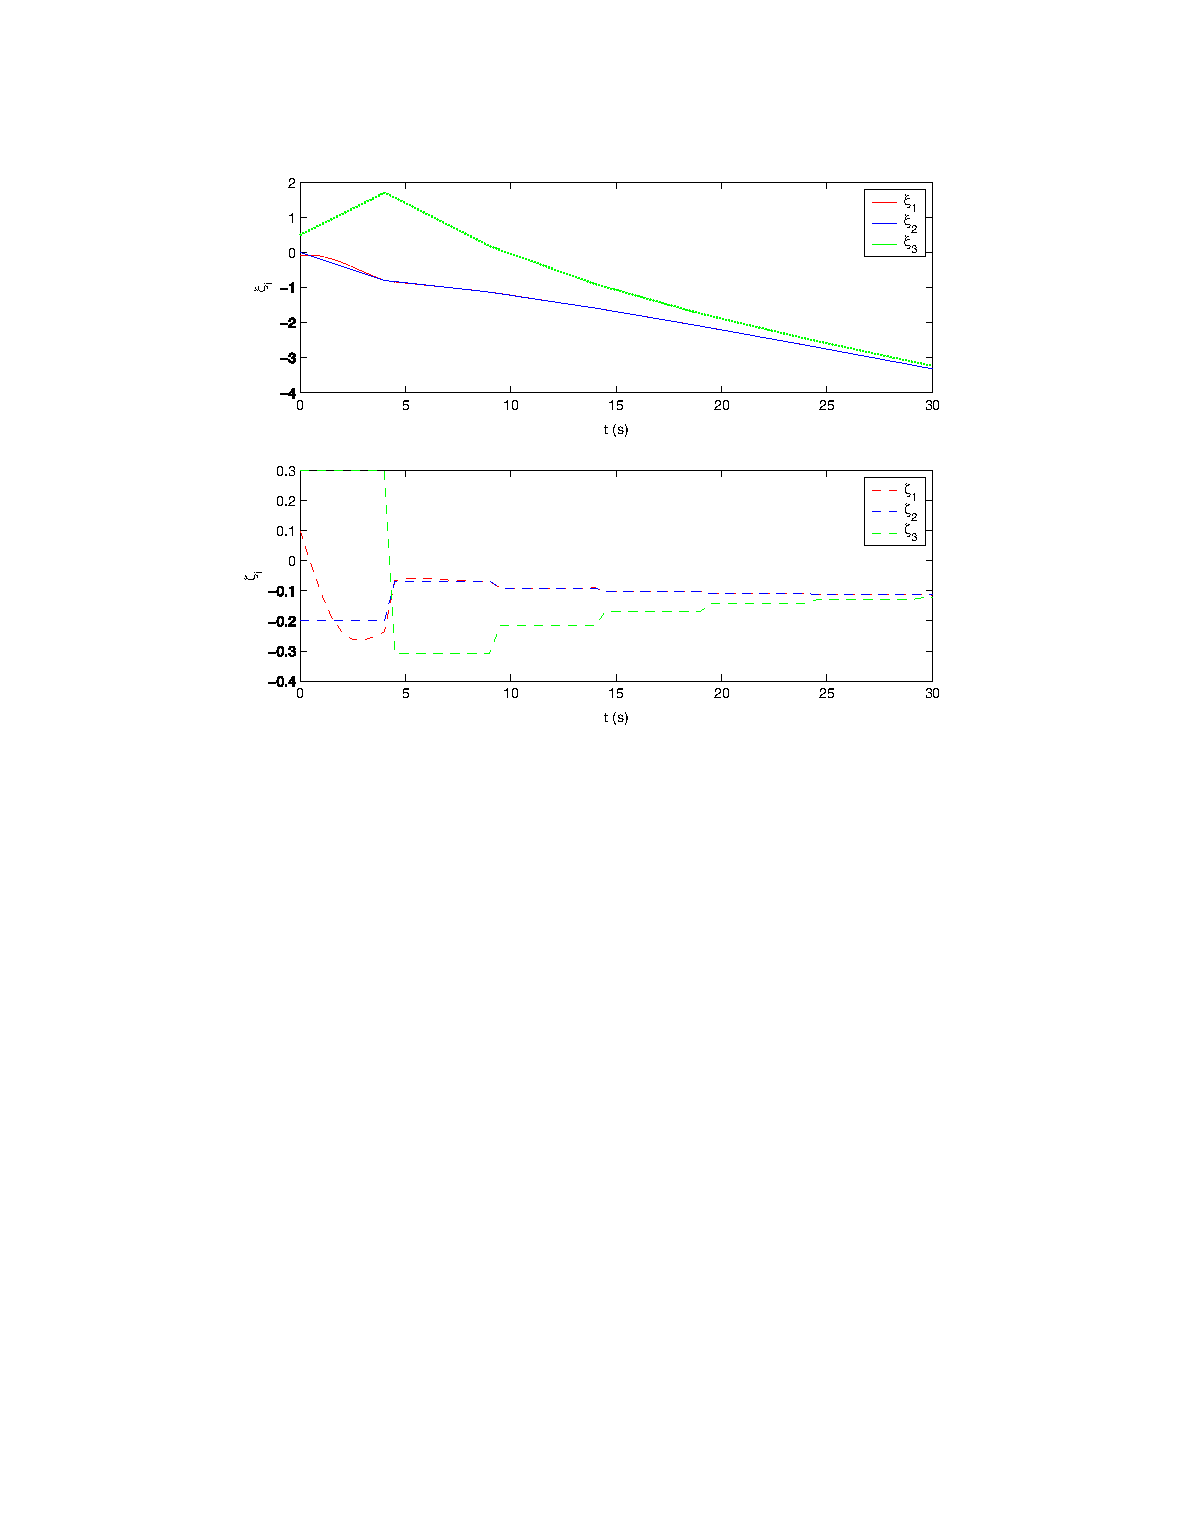
\includegraphics[height=6cm]{images/Switch2.pdf}
	\end{center}
	\vskip 0.3cm
 \end{column}

 \begin{column}{.30\textwidth}
	 In contrast, if we increase the gain $\gamma_2$ to be 10, 
	 {\textcolor{green!40!black}{\fontsize{13}{15}\textbf{consensus can be achieved asymptotically}}}.
 \end{column}
\end{columns}
\vskip 0.3cm

\end{frame}

%%%%%%%%%%%%%%%%%%%%%%
\begin{frame}{Switching graph topology}

\begin{columns}
 \begin{column}{.70\textwidth}
	\begin{center}
		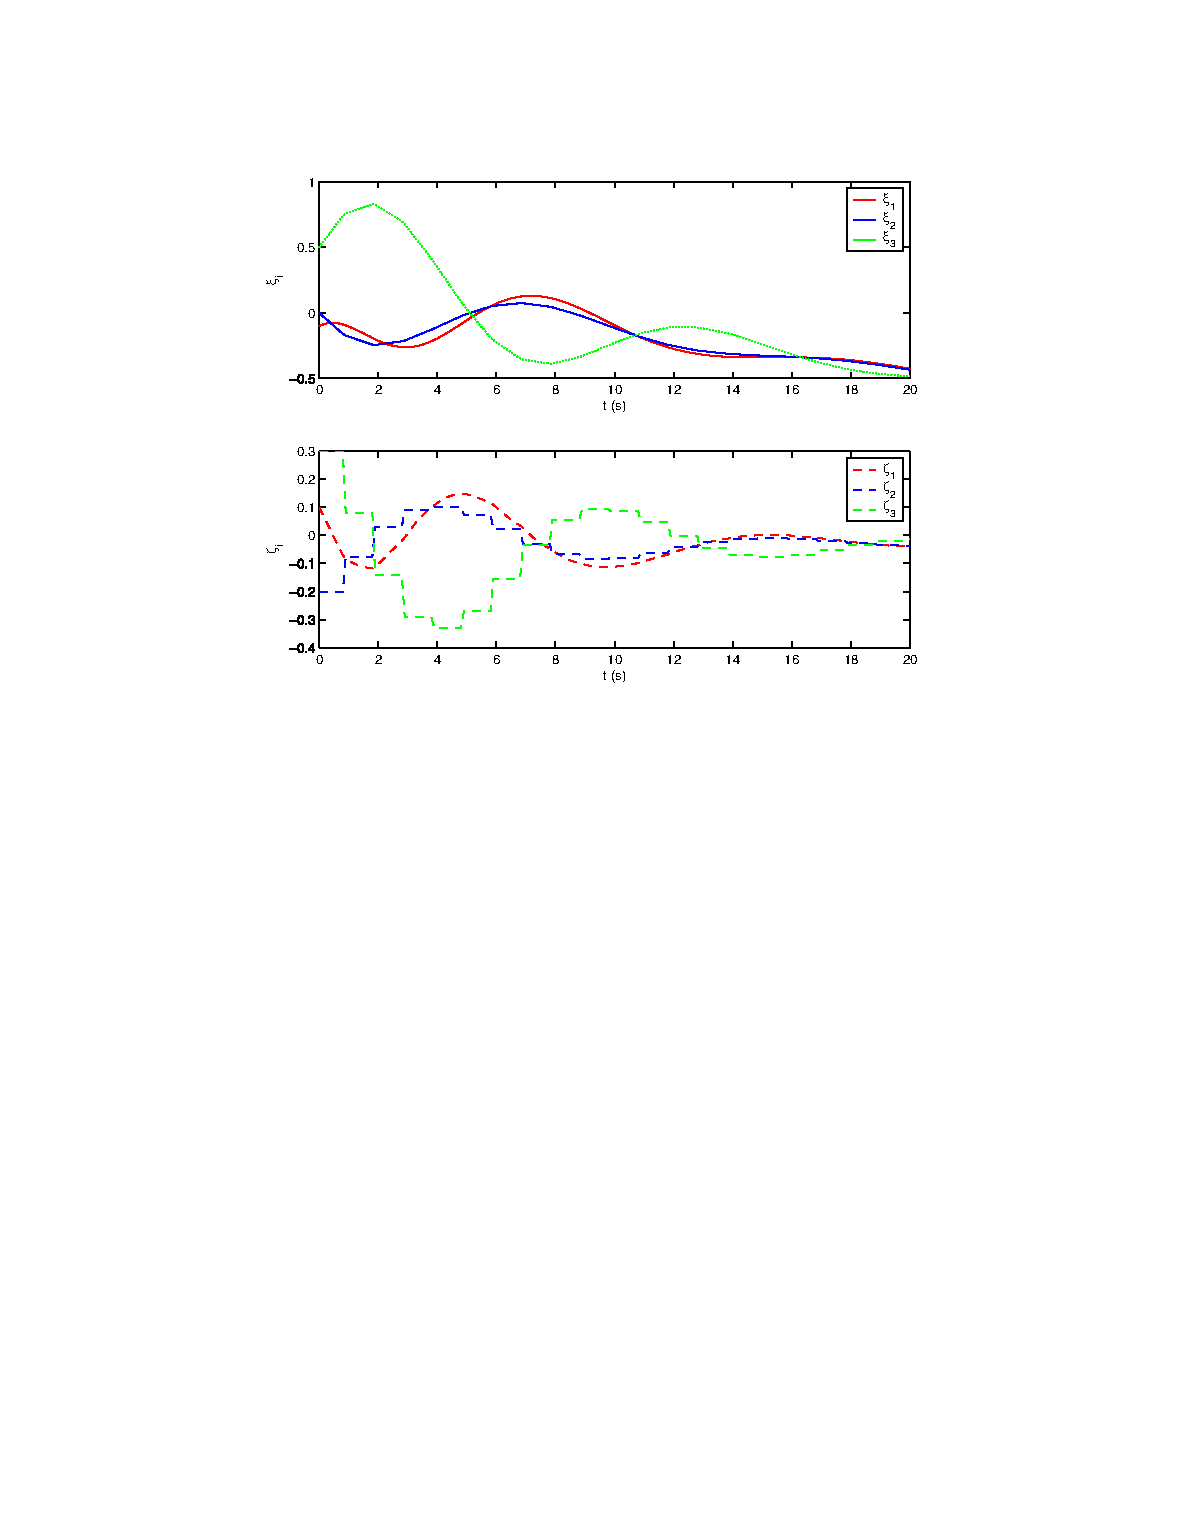
\includegraphics[height=6cm]{images/Switch3.pdf}
	\end{center}
	\vskip 0.3cm
 \end{column}

 \begin{column}{.30\textwidth}
	 Alternatively, if we reduce the length of each time interval to be 1 s,
	 {\textcolor{green!40!black}{\fontsize{13}{15}\textbf{consensus can be achieved asymptotically}}}.
 \end{column}
\end{columns}
\vskip 0.3cm

\end{frame}

%%%%%%%%%%%%%%%%%%%%%%
\begin{frame}{Switching graph topology}

\begin{columns}
 \begin{column}{.70\textwidth}
	\begin{center}
		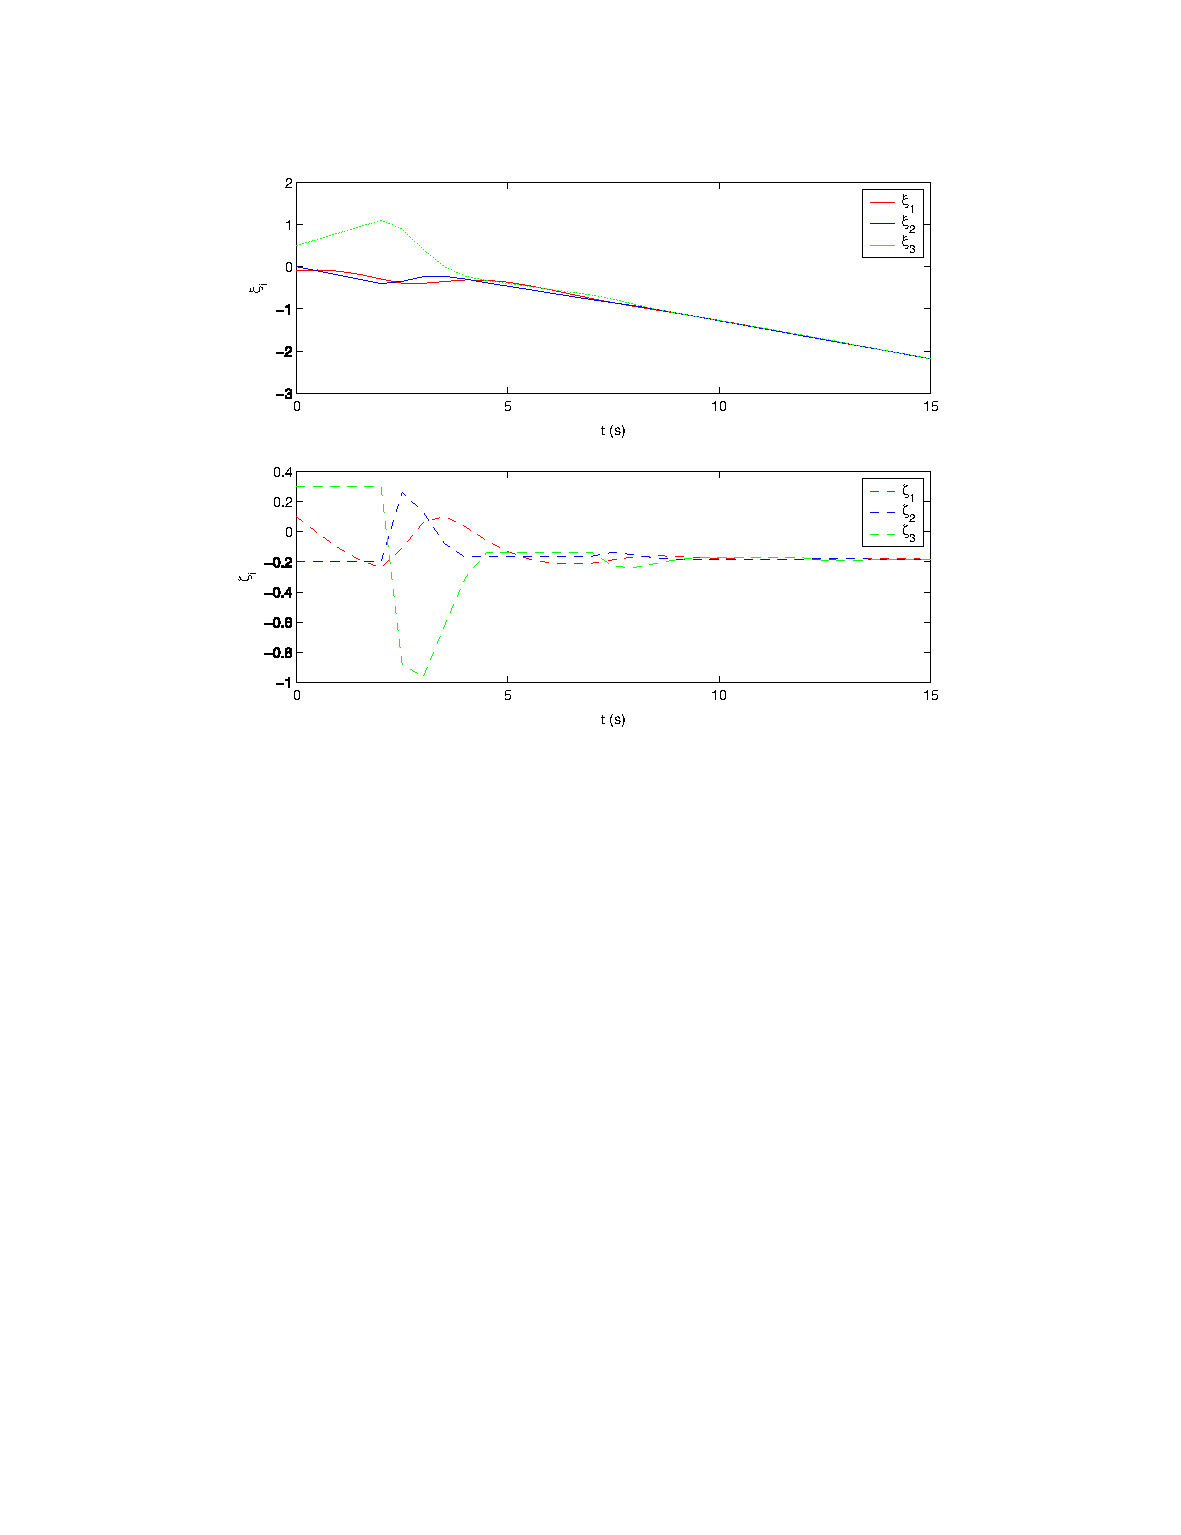
\includegraphics[height=6cm]{images/Switch4.pdf}
	\end{center}
	\vskip 0.3cm
 \end{column}

 \begin{column}{.30\textwidth}
	 In addition, if we let the information exchange topology be $G_1$ during 50\% of the time 
	 and be $G_2$ during the rest of the time with an interval of 5 s,
	 {\textcolor{green!40!black}{\fontsize{13}{15}\textbf{consensus can be achieved asymptotically}}}.
 \end{column}
\end{columns}
\vskip 0.3cm

\end{frame}

%%%%%%%%%%%%%%%%%%%%%%
\begin{frame}{Switching graph topology}

\begin{columns}
 \begin{column}{.70\textwidth}
	\begin{center}
		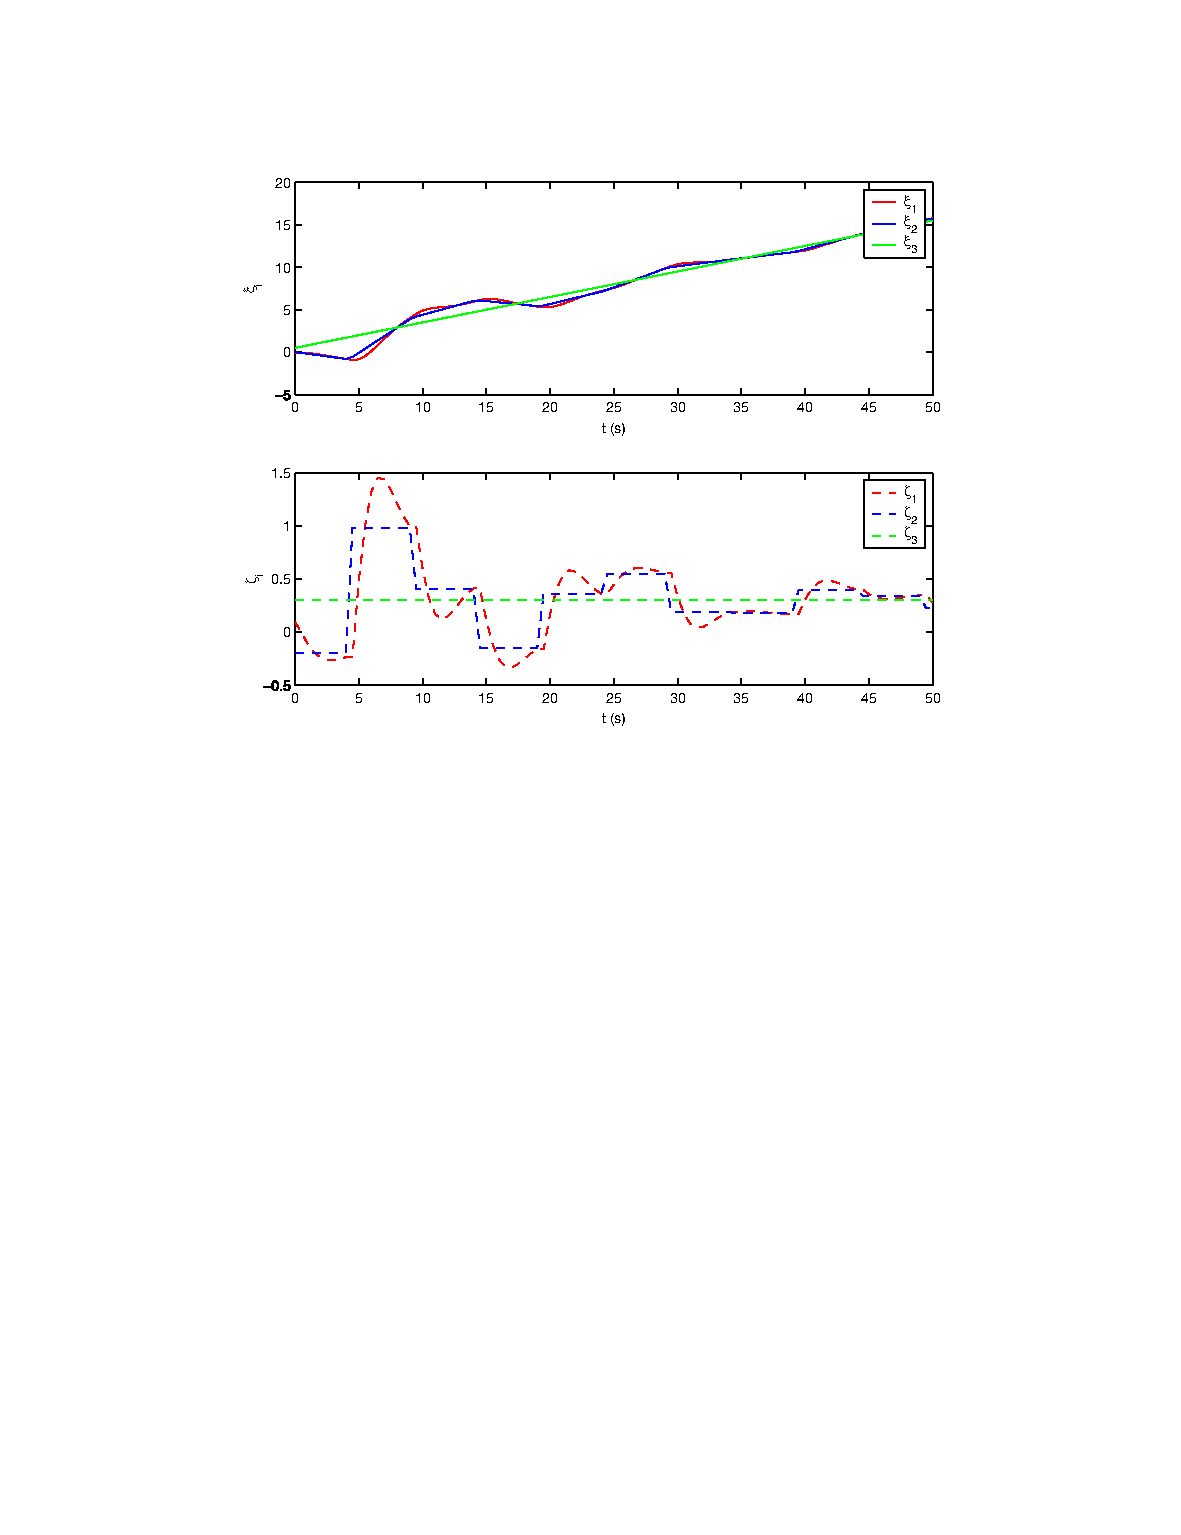
\includegraphics[height=6cm]{images/Switch5.pdf}
	\end{center}
	\vskip 0.3cm
 \end{column}

 \begin{column}{.30\textwidth}
 	\vskip 0.3cm
	 Next, at each time interval of 5 s, we let the exchange topology be $G_1$ during 90\% of the time 
	 and be $G_3$ during the rest of the time. 
	 Note that $G_1 \cup G_3$ has a (directed) spanning tree and that graph $G_3$ is only a subset of graph $G_2$.
 \end{column}
\end{columns}
{\textcolor{green!40!black}{\fontsize{13}{15}\textbf{Consensus can be achieved asymptotically}}} even if graph $G_3$ has less information exchange than graph $G_2$.

\end{frame}